\documentclass[12pt]{article}  
\usepackage{tikz} % new grad package
\usepackage[all, arc, poly ]{xy}
\usepackage{tkz-graph}
\usepackage{latexsym,amsmath}
\voffset=-.8cm
\hoffset=-2cm
\setlength{\textheight}{22.60cm}
\setlength{\textwidth}{14.00cm}
\pagestyle{myheadings}
\newtheorem{q} {Q}
\newcommand{\beq}{\begin{q}}
\newcommand{\eq}{\end{q}\newpage}
\newcommand{\df}{\displaystyle\frac}
\markright {Dr. Petrescu CCP MATH263 Homework 5}
\begin{document}
{\bf Homework 1 Discrete Mathematics II} \vskip0.2cm
\vskip.1cm{\bf Show all your work to get credit. }  \vskip0.2cm 
{\bf Name}: \rule{8cm}{.01cm}\hspace*{0.2cm} {\bf Due Date}: \underline{02/21} \vskip.5cm
%%%questions
\beq For which values of n are these graphs bipartite? \\a) $K_n$\hskip3cm b) $C_n$\hskip3cm c) $W_n$\hskip3cm d) $Q_n$ \eq
\beq A simple graph is called regular if every vertex of this graph has the same degree. A regular graph is called $n- regular$ if every vertex in this graph has degree $n$.  For which values of $n$ are these graphs regular?\\ a) $K_n$\hskip3cm b) $C_n$\hskip3cm c) $W_n$\hskip3cm d) $Q_n$\eq
\beq The complementary graph $\overline G$ of a simple graph G has the same vertices as $G$, however, if two vertices are adjacent in $\overline G$ if and only if they are not adjacent in $G$. Describe each of these graphs. \\ a) $\overline K_n$ \hskip3cm b) $\overline C_n$ \hskip3cm c) $\overline W_n$ \hskip3cm d) $\overline Q_n$ \eq
\beq {\label{q2} Write the adjacency and then incidence matrix for the following graph:\vskip.6cm 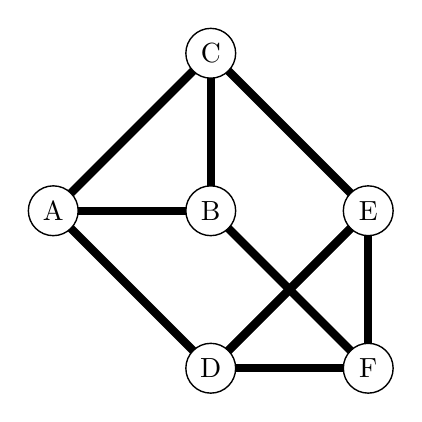
\begin{tikzpicture} \SetGraphUnit{2} \SetUpEdge[lw=3pt] \Vertex{A} \EA (A){B}  \NO (B){C} \SOEA (B){F}  \SO (B){D}     \EA (B){E}   \Edges(A,B,C,A,D,E,F, B,C,E,D,F)  \end{tikzpicture}   \eq
\beq  Create a graph isomorphic, but different than, to  the graph in question \ref {q2}'s graph .   \eq
%%%questions
\end{document}